\documentclass[12pt]{article}
\usepackage{fancyhdr}
\usepackage{datetime}
\usepackage{enumitem}
\usepackage{amsmath}
\usepackage{graphicx}
\graphicspath{ {images/} }
%\usepackage{showframe}

%custom variables
\newdate{date}{16}{09}{2016}
\newcommand{\hwNum}{1}


%header
\pagestyle{fancy}
\lhead{Daniel Andronov}
\chead{\thepage}
\rhead{EC441: Homework \hwNum{}}
\cfoot{\thepage}

\fancyheadoffset[LO,RE]{1pt}
\fancyheadoffset[RO,LE]{1pt}

%titlepage
\title{EC441: Homework \hwNum{}}
\author{Daniel Andronov}
\date{\displaydate{date}}

%addition settings
\topmargin=-0.45in
\evensidemargin=0in
\oddsidemargin=0in
\textwidth=6.5in
\textheight=9.0in
\headsep=0.25in

\begin{document}
\maketitle
\newpage

\section{Textbook Problems}
Problems from the book

\paragraph{P.4\\}
\textbf{Solution:}
\begin{enumerate}[label= \alph*)]
\item 16 maximum possible connections given that the switches are able to support atleast 4 hosts each.
\item 8
\item Yes, for any given link, allow two circuits to be reserved for the AC connectionsn \& two for BD connections. Thus, becuse there are only 2 paths for each connectin, there will be 4 total circuits reserved for both AC \& BD connections.
\item From parts a \& b, m is simply $frac{Ls}{R}$.
\end{enumerate}                          

                                                                                                                                                                                                                                   
\paragraph{P.6\\}                                                                                                                                                      
\textbf{Solution:}
\begin{enumerate}[label = \alph*)]
\item $d_{prop} = m/s.$
\item $d_{trans} = L/R.$
\item $d_{total} = frac{L}{R} + frac{m}{s}.$
\item It is just about to leave A.
\item Some where on the link.
\item Already arrived at B.
\item given L = 120 b, R = 56 Kbps, and s = $2.5\cdot10^8 m/s$, from part a \& b it is obvious that $m = Ls/R$. So,\\
$$m = \frac{Ls}{R} = \frac{120 bits\cdot2.5\cdot10^8 m/s}{56\cdot10^3 bps}= $$\\
$$5.357\cdot10^5 m = 535.7\cdot km = 540 km (2 s.f.).$$
\end{enumerate}                

                                                                                                                                         
\paragraph{P.8\\}                                                                                                                                                      
\textbf{Solution:}
\begin{enumerate}[label = \alph*)]
\item 3Mbs/150Kbps = 20 total connections at maximum.
\item 0.1 or 10\%.
\item Let $X(120, 0.1)$ be a binomal random variable representing the number of users transmiting, then the chance there are n users transmitting is,\\
$$P[X = n] = {120 \choose n}0.1^n0.9^{120-n}.$$
\item From the above equation, $P[X=21] = 0.00414$ (3 s.f.).
\end{enumerate}

                                                                                                                                              
\paragraph{P.13\\}                                                                                                                                                     
\textbf{Solution:}
\begin{enumerate}[label = \alph*)]
\item The first packet will ahve no queueing delay, the second will wait L/R, the third 2L/R, the fourth 3L/R, and so on and so forth. Let $\mu_q$ be  the average queue delay per packet. So,\\
$$\mu_q = \frac{1}{N}\sum_{i = 1}^{N-1}\frac{iL}{R} =\frac{L}{NR}\frac{(N-1)N}{2} = \frac{L(N-1)}{2R}. $$
\item If N packets arrive simultaneously at the link, it would take $\frac{LN(N+1)}{2R}$ sec to disperse. This is vastly larger than the interval at which such N such packets arrive, $\frac{LN}{R}$. Thus, the queue would fill up and packets would be lost. If the queue is infinite, then the average queue time would go to infinity. If the queue size could fit $Q$ packets, then the average wait time would be $\frac{L(Q-1)}{2R}$, and the packets that didn't make it to the queue would be lost.
\end{enumerate}


\paragraph{P.21\\}                                                                                                                                                
\textbf{Solution:}
If only one path able to be used, then the maximum throughput would be $min\{ R^k_1, R^k_2,...,R^k_N\}$, or the mininum rate out of all the links on the given path, $k$.\\If all the paths are usable, then the maximum through put the largest minimum link out of all the paths, or $min\{\ min\{R^1_1, R^2_2,...\}, min\{R^2_1, R^2_2,...\},...,min\{R^M_1, R^M_2,...R^M_N\}\ \}$. 


\paragraph{P.22\\}                                                                                                                                                     
\textbf{Solution:}
\begin{enumerate}[label = \alph*)]
\item $P[ \ packet\ received\  ] = 1 - p$.
\item $n$, average number of re-transmitts, $ = 1/p$.
\end{enumerate}

                                                                                                          
\paragraph{P.23\\}                                                                                                                                                     
\textbf{Solution:}
\begin{enumerate}[label = \alph*) ]
\item The time between the arrival of the last bit of the first packet and that of the second, is the time it takes for the the second packet to arrrive wholly at the destination or the transmission time, $t_{xmit} = L/R_s$. 
\item Yes, as $R_C<R_S$, the first packet would have to slow down, so that the second packet would begin to approach the first. In order have the minimal T, the first packet must completely pass through the queue by the time the second packet arrives at the link. So,\\
\
$$t_{prop} + t_{xmit} + t_{queue} = T + t_{prop} + t_{xmit}$$
$$T = t_{queue} = \frac{L}{R_C}$$
\end{enumerate}

                                                                                                                                             
\paragraph{P.25\\}                                                                                                                                                     
\textbf{Solution:}
\begin{enumerate}[label = \alph*)]
\item The bandwidth-delay product,\\
$$R\cdot d_{prop} = 2Mbps \cdot \frac{ 20,000 km }{ 2.5\cdot 10^8 meters/sec } = \frac{4}{2.5\cdot 10 } Mb$$
$$= 0.16\ Mb = 160\ Kb.$$
\item 160 Kb.
\item The bandwidth-delay product is a measure of how many bits can fill the link.
\item $w_b$, the width of a bit would be $20,000km/160Kb = 125 m$. The width of a football is 109.1 meters long in comparison, which is to say, a bit on this link is longer than a football field.
\item $w_b$, the width of a bit can be defined as,\\
$$w_b = \frac{m}{R\cdot \frac{m}{S} } = \frac{s}{R}$$
\end{enumerate}

                                                                                                                                            
\paragraph{P.33\\}                                                                                                                                                     
\textbf{Solution:}
The transmission time for any packet in this scenario, $t_{xmit} = \frac{S + 80}{R}$. The first packet will take $3t_{xmit}$ to arrive at the destination, B. Afterwards the rest of the packets, of which there are $\frac{F}{S}-1$, will regularly arrive at intervals of $t_{xmit}$. So the rest of the packets will take $(\frac{F}{S} - 1 )t_{xmit}$. So, total transmission delay will be,\\
$$t_T = 3t_{xmit} + \Bigg(\frac{F}{S} - 1\Bigg )t_{xmit}$$
$$=\Bigg(\frac{F}{S} + 2\Bigg)t_{xmit}$$
$$=\Bigg(\frac{F}{S} + 2\Bigg)\frac{S + 80}{R}$$
Then to minimize $t_T$, we take the derivated with respect S and solve for S.First, expanding $t_T$.\\
$$\frac{dt_T}{dS} = \frac{d}{dS}\Bigg( \frac{F}{R} + \frac{80F}{SR} + \frac{2S}{R} + \frac{160}{R}\Bigg )$$
$$ = \frac{-80F}{RS^2} + \frac{2}{R}.$$.
This minimum S is achieved when $\frac{dt_T}{dS}$ is zero. \\
$$ 0 = \frac{-80F}{RS^2} + \frac{2}{R}$$
$$\frac{2}{R} = \frac{-80F}{RS^2}$$
$$S^2 =40F \Rightarrow S = \sqrt{40F}.$$
Thus the minimal transmission delay is when the packets are of size $\sqrt{40F}$.


\section{Additional Questions}

\paragraph{Additonal Question 1\\}
\textbf{Part I, Solution: }
\begin{enumerate}
\item Link 1,\\
$$t_{l1} = t_{prop1} + t_{xmit1} = 1ms + \frac{10^4}{10^6}sec = 11ms.$$\\
Link 2,\\
$$t_{l2} = t_{prop2} + t_{xmit2} = 2ms + \frac{10^4}{2\cdot 10^6}sec = 7ms.$$\\
So, in total, there will be $t_{l1} + t_{l2} = 18ms$ of delay.
\item If ten equal sized packets were used instead then,\\
$$l_1 = t_{prop1} + 10( t_{xmit1} ) = 1 ms + 10( \frac{10^3}{10^6} ) = 11ms.$$\\
$$l_2 = t_{prop2}  + 10(t_{xmit2} ) = 2ms + 10( \frac{10^3}{5\cdot10^6} )= 7ms.$$\\
$$total delay = 18 ms.$$
\end{enumerate}
\textbf{Part II, Solution:\\}
\begin{enumerate}
\item First we calculate the overall delays per packet in both links, without the queue delay.
$$t_{l1} = 2ms + \frac{2.5\cdot10^3 b}{2Mbps} = 127ms.$$
$$t_{l2} = 1ms + \frac{2.5\cdot10^3 b}{1Mbps} = 251ms.$$
The queue time, would be the time it takes for a packet to full enter the second link  from the switch, equvalent to $L/R_{l2} = 250ms$. Now we can create a table, tracking the times of when each pack leaves the switch, counting in total time.
\begin{center}
	\begin{tabular}{ | l | l | l | } 
	\hline
	Packet & Packet arrives at S (ms) & Packet Leaves S (ms) \\ \hline
	1 & 127 & 377 \\ \hline
	2 & 254 & 504 \\ \hline
	3 & 381 & 631 \\ \hline
	4 & 508 & 758 \\ \hline
	\end{tabular}
\end{center}
From here it is very simple to generate the graph, shown below. 
\begin{figure}[h]
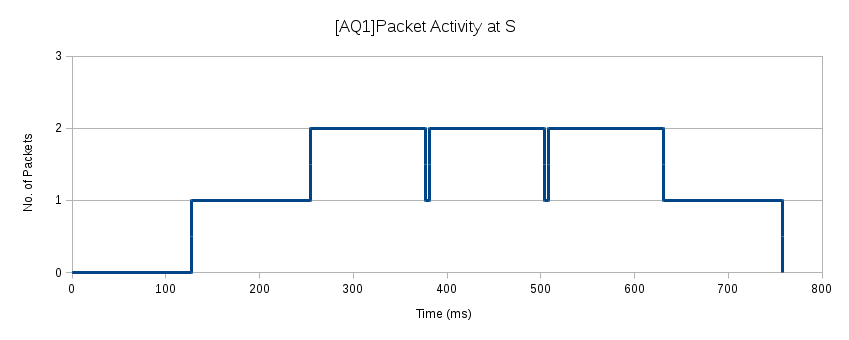
\includegraphics[width=\textwidth, scale = 0.25]{AQ1_graph}
\end{figure}

\item From the above graph, it is 758 ms after the first packet in sent that the final packet leaves the the queue. So we only need to account for the total delay of the final link in order to obtain the total delay for the whole message. Thus $t_{total} = 758ms  + 251ms = 1009ms$ total delay time.
\end{enumerate}

\paragraph{Additional Question II\\}
\begin{enumerate}[label = \alph*)]
\item \$300 million. [ bloomberg.com ]
\item The Hibernia Expresses is reported to be 5.2 milliseconds faster than the previous connection. [bloomberg.com]
\item The prevous path length was reduced by 310 miles by very carefully planning a the shortest route from one seaboard to the other. [bloomberg.com]
\item Video streaming, Voice chat, stock trading. [bloomberg.com]
\end{enumerate}

\end{document}
This is never printed